%% artigo-exemplo.tex

\documentclass[a4paper]{IEEEtran}
\usepackage[utf8]{inputenc}
\usepackage[colorlinks=true]{hyperref}
%\usepackage{latin}
\markboth{MIEEC Dissertation Exams---September 2021}{}
%\usepackage[portuguese]{babel}

\ifCLASSINFOpdf
  \usepackage[pdftex]{graphicx}  
\else
  \usepackage[dvips]{graphicx}
\fi

\renewcommand{\footnoterule}{\noindent\rule{0.5\columnwidth}{0.5pt}\vspace*{3pt}}

\begin{document}

% Título (usar \\ para quebra de linha)
\title{Real-time Ethernet networks: a practical approach to cycle time influence in control applications}


% author names and affiliations
% use a multiple column layout for up to three different
% affiliations
\author{\IEEEauthorblockN{Simão Amorim$^*$}%
\thanks{$^*$\href{mailto:up201605618@edu.fe.up.pt}{up201605618@edu.fe.up.pt}}
\IEEEauthorblockN{Paulo Portugal (supervisor)$^\dag$}%
\thanks{$^\dag$\href{mailto:pportugal@fe.up.pt}{pportugal@fe.up.pt}}
%\IEEEauthorblockN{3� Autor (co-orientador)$^\ddag$}%
%\thanks{$^\ddag$Contacto co-orientador}
}
% make the title area
\maketitle

% \markboth{Uma parte}{Outra parte}

\begin{abstract}
  We live in an increasingly digital and computerised world where there is a constant need for interconnection between everything and everyone.
  Ethernet networks quickly became the communication standard in office and home environments, but their adoption in the industrial environment has been much slower.
  Modern automation and robotic systems do not escape the accelerated need for constant interconnection and, therefore, it is necessary to adapt them, taking into account their real-time requirements.
There are several well-established real-time Ethernet network solutions on the market, but we find the same gap on all of them: the scarcity of educational and demonstration equipment.
  This document aims at providing a quick overview of the most important concepts and results covered on the main document.
\end{abstract}

\begin{IEEEkeywords}
Distributed Control System, EtherCAT, network cycle time.
\end{IEEEkeywords}

\section{Introduction}

\IEEEPARstart{W}{ith} the emergence of digital communication networks, some manufacturers started to introduce fieldbuses into the industry.  These were originally simple networks capable of interconnecting all nodes into a single shared communication medium.

As industrial processes grew in complexity, the amount of data that needed to be shared between nodes also increased.
The existing fieldbuses did not provide enough data throughput for more complex systems.
Fast communication networks such as Ethernet started to become potential targets for the industry due to their data
transfer capabilities, but the methods employed to achieve such higher transfer speeds meant there was no determinism in message deliveries.
Some newer fieldbuses based on the Ethernet started to emerge, such as Ethernet/IP, EtherCAT or PROFINET.

Technology advancements popularised the usage of Distributed Control Systems (DCS) that rely on communication networks for the exchange of information.

\section{Real-time Ethernet networks}
As  most  applications  that  control  industrial  processes  have  some  sort  of  real-time  requirements,  the introduction of an Ethernet network into the control system needs not to disrupt its real-time characteristics.
As such, Real-Time Industrial Ethernet networks have strict timing requirements which makes the usage of common Ethernet not adequate.

Several standard approaches have been defined for how to achieve deterministic communication.
Three different approaches have been explored in depth by describing the key concepts on their basis.
These were named ‘Top of TCP/IP’, ‘Top of Ethernet’ and ‘Modified Ethernet’ \cite{rte:rte-for-automation}.

The first category implements mechanisms on top of the TCP/IP protocol stack, without any modifications applied to it.
Industrial networks such as Modbus/TCP and EtherNet/IP adopted this type of approach.

The second category of RTE networks called ‘On top of Ethernet’ implement a dedicated protocol stack on top of the Ethernet frame, and each one of them specifies a different Ethertype field.
Examples of solutions following this approach are the PROFINET CBA and Ethernet for Plant Automation.

The third category, unlike the previous two, provides a modified Ethernet protocol or hardware.
As a result, it becomes mandatory for solutions that aim for hard real-time performance to employ hardware modifications on the devices or network infrastructure.
Networks such as SERCOS, EtherCAT and PROFINET IO follow this approach.

\subsection{EtherCAT}
The EtherCAT protocol employs a master/slave architecture.
Only the master device is allowed to initiate transmissions and it fully controls the its slaves.
The commands issued by the master evoke responses from the slave devices.

The communication is based on simple Ethernet telegrams encapsulating EtherCAT frames.
The telegrams are identified via the Ethertype field on the Ethernet header.
The EtherCAT frame is composed of an EtherCAT header and one or more EtherCAT commands.
Because EtherCAT frames can contain several commands, the master device can address several slaves using a single frame.

Slave devices receive a telegram, process it and then forwards it to the next slave device on the ring.
If a certain slave device determines it is being addressed by an EtherCAT command, the data is retrieved and/or put into the frame on-the-fly, as the frame is traversing it.
After the last device on the ring has received and processed the frame, it gets sent back to the master device so it can process the responses to the commands it sent \cite{technology:rte2}.

\section{System Architecture}
With our aim being the influence of network cycle time on control applications, it's imperative for us to use an architecture that resembles a Distributed Control System (DCS).
It only makes sense to evaluate such influence on systems where it is applicable, meaning, we must replicate a real world case where the usage of an RTE network might actually influence the system performance.

The main objective is to develop a conceptual distributed control system capable of producing experimental data that demonstrates the impact that the communication network's cycle time has on control applications.
The system will be designed to operate on two different modes: local control and remote control.

With the first configuration (local control), the field device will receive only the set-point values from the RTE network and then perform the position/velocity control of the motor using an internal control algorithm.
This will generate a baseline dataset of control performance, which is expected to barely be affected by the network cycle time.

The second configuration (remote control) will use the field device as a simple servo drive, without using its internal control algorithm.
It shall receive the velocity reference to be applied to the motor from the RTE network and send back the decoded position/velocity, acquired from the motor's incremental encoder, through the same network, as a feedback variable.
This will mean the control loop will be closed on the remote processing unit, making this loop's output and feedback values traverse the RTE network.
It's expected for this configuration to be mildly affected by the network cycle time, even though we will probably need to use unusually large values of this parameter to obtain relevant changes in the control performance.

The hardware for the slave device has also been chosen carefully, taking into account all required and even desirable functions and characteristics.
An overview of the slave device architecture is shown in \autoref{fig:slave-architecture}.

\begin{figure}[ht]
  \centering
  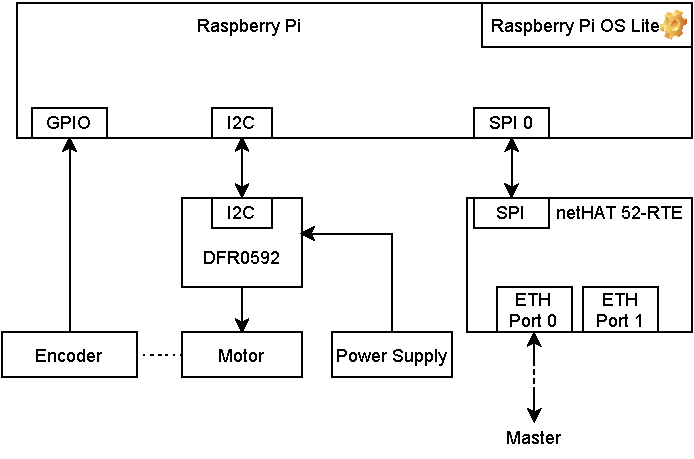
\includegraphics[width=.8\linewidth]{slave_architecture.pdf}
  \caption{Overview of the slave device architecture}
  \label{fig:slave-architecture}
\end{figure}

\section{Results}
The following \autoref{tab:step-analysis} shows a summarised overview of the data analysis performed on the experiment data we gathered.

We have performed three tests with each control mode using three different network cycle periods: 5ms, 10ms and 20ms, which are half, full and double of the chosen processing period (10ms), respectively.

Looking at the resulting data, especially comparing the data for the test cases when the network cycle time is larger that the control period (20ms test case) the system presents a much less stiff response during remote operation than during local control.
This is evidence that, in fact, network cycle time truly influences distributed control systems.

Motion control systems require cycle times not larger that 1ms, with jitter values not exceeding 1$\mu$s \cite{rte:rte-for-automation}.
When working with such small cycle times, any variation on the control loop cycle times can cause it to become unstable and, in more extreme cases, turn the whole system uncontrollable.

\begin{table}[h]
	\centering
	\caption{Step-response evaluation of each test case (summarised)}
	\label{tab:step-analysis}
	\begin{tabular}{|c|c|c|c|c|c|}
		\hline
		Test Case   & rise-time (s) & settling-time (s) & overshoot (\%) \\
		\hline
		local-5ms   & 0.0366 & 1.8327 & 11.1124 \\
		\hline
		remote-5ms  & 0.0597 & 1.9769 & 30.555 \\
		\hline
		local-10ms  & 0.0544 & 5.1091 & 0.0301 \\
		\hline
		remote-10ms & 0.0434 & 5.1745 & 24.3232 \\
		\hline
		local-20ms  & 0.0472 & 4.7729 & 5.5528 \\
		\hline
		remote-20ms & 0.6024 & 5.1745 & 0.0902 \\
		\hline
	\end{tabular}
\end{table}

\section{Conclusion}

The experimental results confirm the validity of the system proposed in this document and provide a good indication that future works based on the presented concept are likely to produce positive results.

Although simple, the developed system and concept have been able to produce results with minimum external influence.
Most times implementing and designing less can mean much more, and the results we obtained are proof of that.
The developed barebones Distributed Control System has allowed us to explore the influence of the network cycle time on control systems.

\section*{Acknowledgements}
I want to thank professor Paulo Portugal for his continuous availability  to provide me with the best and most informed feedback possible, during all stages of the project.

I would also like to thank my family for putting up with my working habits and routines while we were all working from home during the COVID-19 pandemic.
Sometimes it wasn't easy to reconcile work and personal life, but these were definitely times where everyone had to adapt to a new reality.

Lastly, I want to dedicate this work to my good friend Ania who helped me get through some rough times on my personal life.

% referências

\bibliographystyle{IEEEtran}
\bibliography{refs}

\end{document}


